\chapter{Trabajo desarrollado}
\thispagestyle{empty}


En este capítulo se explican las funcionalidades básicas del simulador desarrollado centradose únicamente en los aspectos más importantes. Para profundizar más sobre estos aspectos debe acudir a los anexos.

\section{Resumen del simulador}
\thispagestyle{empty}

Se trata de un sistema de colaboración abierta distribuida que permite configurar distintos escenarios con objetos móviles y estáticos sobre mapas de ciudades reales obtenidos a partir del servicio de mapas de OpenStreetMap. 

El simulador de escenarios está basado en el simulador Mavsim desarrollado por el Grupo de Sistemas de Información Distribuidos de la Universidad de Zaragoza utilizado para la simulación de VANETs en el cual hay muchos vehículos distribuidos en una amplia zona geografica.

\begin{figure}[H]
\centering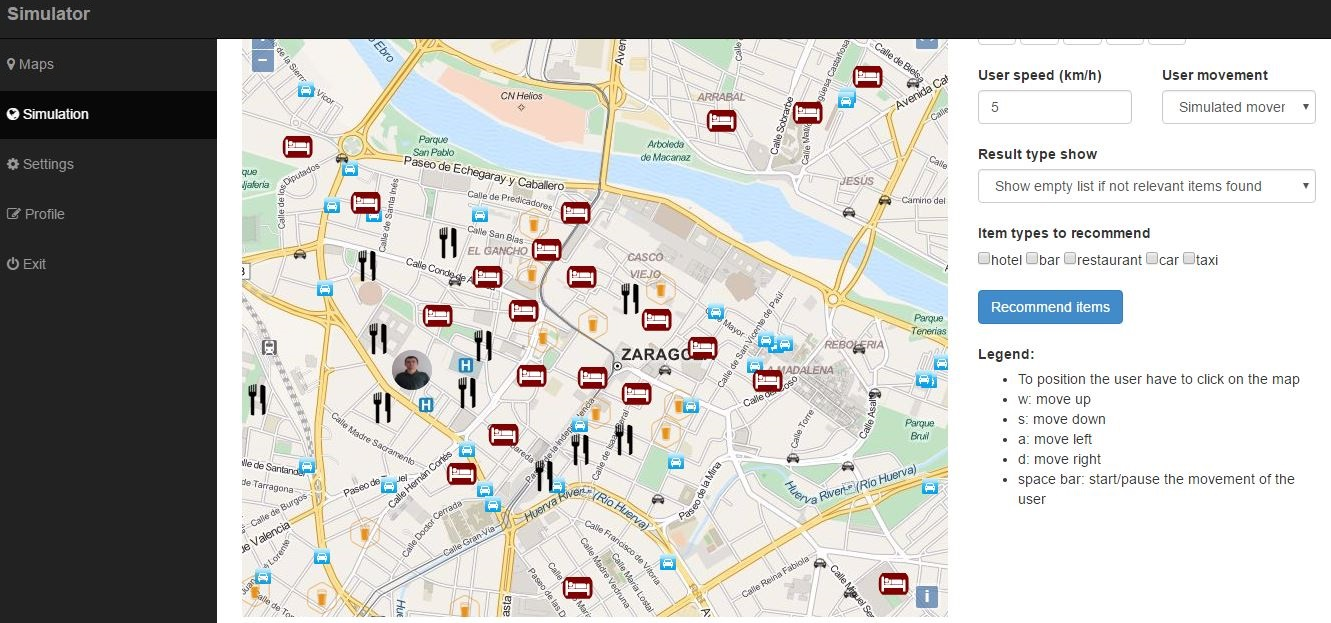
\includegraphics[width=0.8\textwidth]{imagenes/resumen-simulador.jpg}
\caption{Simulación en Actur, Zaragoza con un solo usuario}
\label{c2_trama}
\end{figure}

Puede ser usado a través de cualquier dispositovo (PC, tablet, móvil etc.) con conexión a Internet y un navegador web. Permite a los usuarios crear sus propios mapas y escenarios. Durante la creación de una escena el usuario elige cual es la cuidad donde se realiza la simulación, el recomendador a utilizar, si el mapa es colaborativo o no, introducir los objetos estáticos y configurar cuales son los objetos móviles y sus rutas. 

Para realizar una simulación el usuario tiene que buscar y seleccionar el mapa y escenario donde moverse tanto para obtener recomendaciones como para realizar votaciones sobre los distintos objetos de este entorno.

\section{Arquictura del sistema}
\thispagestyle{empty}

\begin{figure}[H]
\centering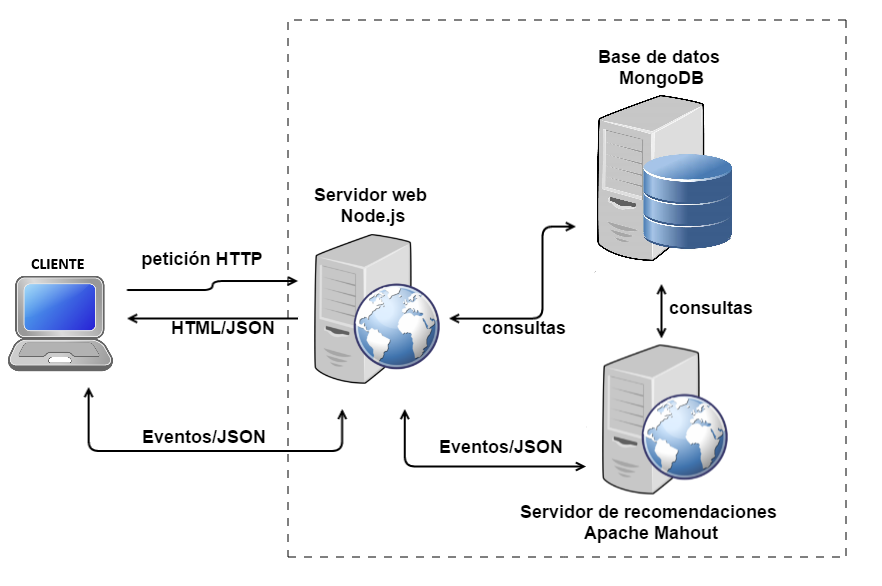
\includegraphics[width=0.9\textwidth]{imagenes/arquitectura-componentes.png}
\caption{Arquitectura de componentes del sistema}
\label{arquitecturaComponentes}
\end{figure}